
%%%%%%%%%%%%%%%%%%%%%%%%%%%%%%%%%%%%%%%%%%%%%%%%%%%%%%%%%%%%%
%%%%%%%%%%%%%%%%%%%%%%%%%%%%%%%%%%%%%%%%%%%%%%%%%%%%%%%%%%%%%
%
%  %%%%%%%  %    %  %%%%%%  %%%%%%  %%%%%%%  %%%%%%%  %%%%%
%  %        %    %  %    %  %     %    %     %        %    %
%  %        %    %  %%%%%%  %     %    %     %        %    %
%  %        %%%%%%  %    %  %%%%%%     %     %%%%%    %%%%%
%  %        %    %  %    %  %          %     %        %    %
%  %%%%%%%  %    %  %    %  %          %     %%%%%%%  %     %
%
%%%%%%%%%%%%%%%%%%%%%%%%%%%%%%%%%%%%%%%%%%%%%%%%%%%%%%%%%%%%%
%%%%%%%%%%%%%%%%%%%%%%%%%%%%%%%%%%%%%%%%%%%%%%%%%%%%%%%%%%%%%

\chapter{Homology and Cohomology}
\label{sec:homology}

\begin{quote}
{\em``The de Rham complex may be viewed as a God-given set of differential equations, whose solutions are the closed forms.... A measure of the size of the space of `interesting' solutions is the definition of the de Rham cohomology.''}
\begin{flushright} --- Raoul Bott and Loring Tu~\cite[p. 15]{bott1982differential} \end{flushright}
\end{quote}

In Section~\ref{subsec:posets} and Chapter~\ref{sec:maps} we worked over arbitrary posets. We did this because it was natural and some applications may need this level of generality. In this section, we eschew this generality and restrict ourselves to posets arising as the face relation of a finite cell complex. This is beneficial not only because cell complexes are of great interest, but because sheaves and cosheaves over them have easily defined cohomology and homology theories.

We will start by describing a simple generalization of cellular cohomology and homology where we have augmented the coefficients by placing vector spaces over individual cells and linear maps between incident cells. This is a generalization in the sense that if one restricts to the case where every cell is assigned the one-dimensional vector space $k$ and all the incident linear maps are the identity, we recover classical cellular (co)homology. However interesting this special case may be, it misses a theory general enough to compute homological invariants of data varying over a cell complex.

The theory presented is combinatorial and computable. One needs only a good working knowledge of linear algebra to be able to use it. However, one can compute cellular sheaf cohomology without understanding it. To clarify the meaning of these computations we adopt a representation-theoretic perspective. This allows us to break up sheaves and cosheaves into the basic building blocks of indecomposable representations of the cell category. Thus, borrowing terminology from the persistent homology community, we use ``generalized barcodes'' to see the topology of data in a wider world of applications. These ideas are be put into practice in Chapters \ref{sec:barcodes}, \ref{sec:nc_coding}, and \ref{sec:sensors}, where many examples are considered.

\section{Chain Complexes and Homology}

\begin{defn}\index{graded vector space}
A \textbf{$\Z$-graded vector space} $V^{\ast}$ is a collection of vector spaces $\{V^i\}_{i\in\ZZ}$ with one for each integer. A \textbf{graded map} is a collection of linear maps $f:V^i\to W^i$. The \textbf{category of $\Z$-graded vector spaces}, $\grVect$, has graded vector spaces $V^{\ast}$ for objects and graded maps for morphisms.
\end{defn}

A (co)chain complex is a graded vector space with extra structure.

\begin{defn}\index{Cochain@(co)chain complex}
A \textbf{cochain complex} consists of a collection of vector spaces called \textbf{cochain groups} $\{V^i\}_{i\in\Z}$ and a collection of linear maps called \textbf{differentials} $d^i:V^i\to V^{i+1}$ that satisfy $d^{i+1}\circ d^i=0$ for every $i\in\Z$. We denote a cochain complex by $(V^{\bullet},d^{\bullet})$. Alternatively said, a cochain complex is a graded vector space equipped with a degree one increasing map that when composed twice gives the zero map.


A \textbf{chain complex} is a cochain complex with different notation. The \textbf{chain groups} $\{V_i\}_{i\in\Z}$ and \textbf{boundary maps} $\partial_i:V_i\to V_{i-1}$ are decorated with subscripts; this is the only difference. The maps satisfy $\partial_{i-1}\circ\partial_i=0$ for every $i\in\Z$. We denote a chain complex by $(V_{\bullet},\partial_{\bullet})$.
\end{defn}

\begin{rmk}
Since chain complexes and cochain complexes are the same thing, merely dressed up in different notation, we will usually just say ``Let $(V^{\bullet},d^{\bullet})$ be a chain complex'' and let the mathematical notation be precise. As an aside, one can also say that a chain complex is \emph{homologically indexed} if it is written as $(V_{\bullet},\partial_{\bullet})$ or \emph{cohomologically indexed} if it is written as $(V^{\bullet},d^{\bullet})$.
\end{rmk}

\begin{rem}
Sometimes we drop the subscript or superscript $\bullet$ and write $(V,\partial)$ or $(V,d)$ to refer to a chain complex or cochain complex. Dropping the superscript can lead to overloaded notation. For example, the expression $d^2=0$ is a synonym for ``$d$ is a differential,'' i.e. $d^{i+1}\circ d^i=0$ for ever $i\in\Z$, but it could also mean that the map $V^2\to V^3$ is zero. This is one of the perils of cohomological indexing for chain complexes, but the ambiguity is resolved by scoping the context. If we are speaking at the high-level of viewing a chain complex as a different sort of structure, then the former interpretation is intended. If we are talking about the particulars of a given chain complex, then the latter is meant. 
\end{rem}

\begin{defn}\index{category!C@$\Ch^{\bullet}(\Vect)$ of chain complexes}
The \textbf{category of chain complexes}, $\Ch^{\bullet}(\Vect)$, has chain complexes for objects, and chain maps $f^{\bullet}:(V,d_V)\to (W,d_W)$ for morphisms, i.e. a collection of maps $f^i:V^i\to W^i$ such that $f^{i+1}\circ d^i_V=d^i_W\circ f^i$.
\end{defn}

There is a natural functor $\iota: \grVect\to\Ch(\Vect)$ that treats a $\Z$-graded vector space as a chain complex with zero differentials, i.e.
\[
\{V^i\}_{i\in\Z} \rightsquigarrow (V^{\bullet},0)
\]
Taking cohomology of a chain complex defines a functor going the other way.

\begin{defn}\index{cohomology}
\textbf{Cohomology} is a functor $H^{\ast}:\Ch(\Vect)\to\grVect$, which takes a chain complex $(V,d)$ and places the quotient vector space 
\[
H^i(V,d):=\ker(d^i)/\im(d^{i-1})
\] 
in degree $i$. Without too much work one can show that a chain map $f^{\bullet}$ induces maps of the associated cohomology spaces $H^i(f):H^i(V,d_v)\to H^i(W,d_w)$, making $H^{\ast}$ into a functor.
\end{defn}

\subsection{The Combinatorics of Cell Complexes and Homology}

The motivation for chain complexes and homology comes from computing invariants of topological spaces. As already indicated, posets can be regarded as topological spaces, but not every poset has the nice structure that the face-relation poset of a cell complex has. This nice structure is what determines whether certain sequence of vector spaces and maps defines a chain complex.

\begin{defn}
We write $\sigma \leq_i \tau$ if the difference in dimension of the cells is $i$.
\end{defn}

\begin{lem}\label{lem:2cells}
 If $\sigma\leq_2\tau$, then there are exactly two cells $\lambda_1,\lambda_2$ where $\sigma\leq_1\lambda_i\leq_1\tau$.
\end{lem}

We want to invent a sign condition that distinguishes these two different sequences of incidence relations.
\[
	\xymatrix{ & \tau & \\ \lambda_1 \ar[ru] & & \lambda_2 \ar[lu]\\ & \ar[lu] \sigma \ar[ru] &}
\]

\begin{defn}[Signed Incidence Relation]\index{incidence relation}
 A \textbf{signed incidence relation} is an assignment to any pair of cells $\sigma,\tau\in X$ a number $[\sigma:\tau]\in\{0,\pm 1\}$ such that 
 \begin{itemize}
 \item if $[\sigma:\tau]\neq 0$, then $\sigma\leq_1\leq _1 \tau$, and
 \item if $\gamma$ and $\tau$ are any pair of cells, the sum $\sum_{\sigma}[\gamma:\sigma][\sigma:\tau]=0$.
 \end{itemize}
\end{defn}

One way to get a signed incidence relation is to choose a \textbf{local orientation}\index{local orientation} (via the homeomorphism of each cell $|\sigma|$ with $\RR^k$) for each cell without regard to global consistency. Then for every pair of incident cells $\sigma\leq\tau$ we have a number $[\sigma:\tau]=\pm1$ given by $+1$ if the orientations agree and $-1$ otherwise.

Another way is motivated by working with regular cell complexes, where we can subdivide so that we have a simplicial complex. We can refer to any cell by a list of its vertices. If we order the set of vertices, then we have a procedure for orienting the cells. A local orientation of a cell $\sigma\in X$ consists of divvying up the set of ordered lists representing $\sigma$ into classes each of which are invariant under even permutations. We can then pick the class with the list of vertices in increasing order as ``the'' orientation. Either method enables us to define a chain complex associated to a cell complex.

\begin{prop}[Cellular Cohomology]\index{cohomology!of a cell complex}
Let $X$ be a cell complex equipped with a sign relation. Let $C^n(X;k)$ be the vector space spanned by the $n$-dimensional calls of $X$. We define a map $\delta:C^n\to C^{n+1}$ on the basis by defining $\delta(\sigma)=\sum_{\tau} [\sigma:\tau]\tau$. Clearly $\delta^2=0$.
\end{prop}

\section{Computational Sheaf Cohomology and Cosheaf Homology}
\label{subsec:comp_homology}

We now provide formulae for computing cellular sheaf cohomology and cellular cosheaf homology that is completely analogous to cellular cohomology.

\subsection{Cellular Sheaf Cohomology}

\begin{defn}[\cite{dihom_1, shepard}]\index{cohomology!of a cellular sheaf!compactly-supported}\index{sheaf!cellular!compactly supported cohomology of}
 Given a cellular sheaf $F:X\to\Vect$ we define its \textbf{compactly supported $k$ co-chains} to be the product\footnote{Here we implicitly assume that $X$ has finitely many cells in a given dimension so products and direct sums agree.} of the vector spaces residing over all the $k$-dimensional cells.
\[
 C^k_c(X;F)=\bigoplus_{\sigma^k}F(\sigma^k)
\]
 These vector spaces are graded components in a complex of vector spaces $C^{\bullet}_c(X;F)$. The differentials are defined by
\[
 \delta^k_c=\sum_{\sigma\leq\tau} [\sigma^k:\tau^{k+1}]\rho_{\tau,\sigma}.
\]
The cohomology of this complex
\[
 \xymatrix{0 \ar[r] & \oplus F(\mathrm{vertices}) \ar[r]^-{\delta_c^0} & \oplus F(\mathrm{edges}) \ar[r]^-{\delta_c^1} & \oplus F(\mathrm{faces}) \ar[r] & \cdots & = C^{\bullet}_c(X;F)}
\]
is defined to be the \textbf{compactly supported cohomology} of $F$, i.e. $H^k_c(X;F)=\ker\delta^k_c/\im \delta^{k-1}_c$.
\end{defn}

\begin{lem}
 $(C^{\bullet}_c(X;F),\delta^{\bullet}_c)$ is a chain complex.
\end{lem}
\begin{proof}
To see why the chain complex condition $\delta_c^{k+1}\delta_c^{k}=0$ is assured, Lemma \ref{lem:2cells} is crucial. This is the very same lemma that proves that ordinary cellular homology is computed via a chain complex. One must now observe that varying data over the cells does not change the result.
\begin{eqnarray*}
 \delta_c\delta_c &=& \sum_{\sigma\leq_1\tau} [\sigma:\tau]\rho_{\tau,\sigma}(\delta_c) \\
 &=& \sum_{\sigma\leq_1\tau} [\sigma:\tau]\rho_{\tau,\sigma}(\sum_{\gamma\leq_1 \sigma} [\gamma:\sigma]\rho_{\sigma,\gamma}) \\
 &=& \sum_{\gamma\leq_1\sigma\leq_1\tau} [\gamma:\tau] \rho_{\tau,\sigma}\rho_{\sigma,\gamma} \\
 &=& \sum_{\gamma\leq_1\sigma\leq_1\tau} [\gamma:\tau] \rho_{\tau,\gamma} \\
 &=& \sum_{\gamma\leq_1\sigma\leq_1\tau} ([\gamma:\sigma_1][\sigma_1:\tau]+[\gamma:\sigma_2][\sigma_2:\tau]) \rho_{\tau,\gamma} \\
 &=& 0
\end{eqnarray*}
\end{proof}

To define the arbitrarily-supported cochain complex associated to a cellular sheaf $F$ on $X$, we simply remove all the cells from $X$ without compact closures and apply the same formula.

\begin{defn}[Ordinary Cohomology]\index{cohomology!of a cellular sheaf}\index{sheaf!cellular!cohomology of}
    Let $X$ be a cell complex and $F:X\to\Vect$ a cellular sheaf. Let $j:X'\to X$ be the subcomplex consisting of cells that do not have vertices in the one-point compactification of $X$. Define the ordinary cochains and cohomology by
\[
	C^{\bullet}(X;F)=C^{\bullet}_c(X';j^*F) \qquad H^i(X;F):=H^i_c(X';j^*F)
\]
\end{defn}

The situation may seem a bit unusual. The naturally defined chain complex computes a more restrictive type of cohomology. To get the standard cohomology, one needs to remove non-compact cells. When we define cohomology via the derived perspective of Section \ref{sec:derived}, this quirk of linear algebra disappears. Ordinary cohomology will fall out naturally using limits and injective resolutions, and compactly-supported sheaf cohomology will require some finesse.

\begin{ex}[Compactly Supported vs. Ordinary Cohomology]
To see why the na\"ive chain complex computes compactly supported cohomology, consider the example of the half-open interval $X=[0,1)$ decomposed as $x=\{0\}$ and $a=(0,1)$. Now consider the constant sheaf $k_X$. To compute compactly supported cohomology, we must first pick a local orientation of our space. By choosing the orientation that points to the right, we get that $[x:a]=-1$. The cohomology of our sheaf is computed via the complex
\[
  \xymatrix{k \ar[r]^{-1} & k},
\]
which yields $H^0_c=H^1_c=0$. If we follow the prescription for computing ordinary cellular sheaf cohomology, then we must remove the vector space sitting over $a$ in our computation. The resulting complex is simply the vector space $k$ placed in degree 0, so $H^0(X;k_X)=k$ and is zero in higher degrees.
\end{ex}

\begin{figure}[ht]
\centering
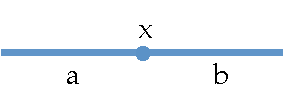
\includegraphics[width=.3\textwidth]{open_interval_p.pdf}
\caption{Minimal Cell Structure on an Open Interval}
\label{fig:open_interval}
\end{figure}

\begin{ex}[Open Interval]
 If we pretended for a moment that the pure stratum $Y=(0,1)$ is a cell complex\footnote{Recall that we require a cell complex to have a one point compactification that is a regular cell complex.} with no other cells, then computing the compactly supported cohomology of the constant sheaf would yield a vector space in degree one and nowhere else, hence $H^1_c(Y;k_Y)=k$.

 To make this example a legitimate example, as in Figure \ref{fig:open_interval}, we place a vertex at $x=1/2$. We call our new cells $a=(0,1/2)$ and $b=(1/2,1)$. If we orient our 1-cells to point to the right, then $[x:a]=1$ and $[x:b]=-1$. Using the lexicographic ordering on our cells to get a basis for $C^1_c(Y;k_Y)$ we can compute explicitly the compactly supported cohomology.
 \[
  \delta^0_c=\begin{bmatrix}1 \\ -1\end{bmatrix} : k_x \to k_a\oplus k_b \qquad \Rightarrow \qquad H^0_c=0 \quad H^1_c=k
 \]
\end{ex}

\subsection{Cellular Cosheaf Homology}

For cellular cosheaves the exact dual construction works, but the terminology is slightly different.

\begin{defn}[Borel-Moore Cosheaf Homology]\index{homology!of a cellular cosheaf!Borel-Moore}\index{cosheaf!cellular!Borel-Moore homology of}
 Let $X$ be a cell complex and let $\hF:X^{op}\to\Vect$ be a cellular cosheaf. Define the \textbf{Borel-Moore homology of} $H_{\bullet}^{BM}(X;\hF)$ to be the homology of the following complex:
\[
 \xymatrix{C^{BM}_{\bullet}(X;\hF) = & \cdots \ar[r] & \oplus \hF(\mathrm{faces}) \ar[r]^-{[e:\sigma]r_{e,\sigma}} & \oplus \hF(\mathrm{edges}) \ar[r]^-{[v:e]r_{v,e}} & \oplus \hF(\mathrm{vertices}) \ar[r] & 0 }
\]
\end{defn}

\begin{defn}[Ordinary Cosheaf Homology]\index{homology!of a cellular cosheaf}\index{cosheaf!cellular!homology of}
	Let $X$ be a cell complex and let $\hF:X^{op}\to\Vect$ be a cellular cosheaf. By discarding all the cells without compact closure, we obtain the maximal compact subcomplex $X'$. If we write $j:X'\hookrightarrow X$ for the inclusion, then we can define the ordinary chain complex to be
	\[
	C_{\bullet}(X;\hF)=C^{BM}_{\bullet}(X';j^*\hF).
	\]
	Applying the definition above gives the ordinary \textbf{cosheaf homology} $H_{\bullet}(X;\hF)$ of a co-sheaf.
\end{defn}

All of the examples of cellular sheaf cohomology dualize to give interesting examples of cellular cosheaf homology. Let us define the functor that performs this operation.
\begin{defn}[Linear Duality]\index{duality!linear}\index{linear duality}
	Let $\widehat{V}: \Shv(X;\vect_k)^{op} \to \Coshv(X;\vect_k)$ be the contravariant equivalence from sheaves to cosheaves, both valued in \emph{finite} dimensional vector spaces, defined as follows:
	\[
		\xymatrix{F(\tau) \ar@{~>}[r] & F(\tau)^*  \ar[d]^{\rho^*_{\tau,\sigma}} & \widehat{V}(F)(\tau) \ar[d]^{r_{\sigma,\tau}} \\
		F(\sigma) \ar[u]^{\rho_{\tau,\sigma}} \ar@{~>}[r] & F(\sigma)^* & \widehat{V}(F)(\sigma)}
	\]
\end{defn}

\begin{lem}
 Taking linear duals preserves cohomology, i.e. $H_i(X;\widehat{V}(F))\cong H^i(X;F)$ and $H_i^{BM}(X;\widehat{V}(F))\cong H^i_c(X;F)$.
\end{lem}

\section{Explaining Homology and Cohomology via Indecomposables}
\label{subsec:rep_thy}

Sheaf cohomology is notoriously difficult to interpret. Every time a successful interpretation is discovered, a cornerstone of a theory waiting to be fleshed out is put into place. For example, the Cousin problems of complex analysis asks whether a meromorphic function with a given divisor (zeros and poles) exists or not. When Cartan and Serre interpreted this problem in terms of sheaf theory, sheaf cohomology groups gave a complete classification and obstruction theory; see~\cite{gray} p. 17. The narrative that falls out of those historical successes is that sheaf cohomology gives calculable obstructions to finding solutions.

However, when the above interpretation fails, we need to compute examples and extract new interpretations. When computing sheaf cohomology, one encounters a plethora of choices that obfuscate the natural meaning of the vector spaces $H^i(X;F)$: picking ordered bases for each $F(\sigma)$, choosing local orientations, computing kernels and quotients, taking representative elements of cohomology or homology, etc. Each of these lead one farther from a workable interpretation of the topology of data.

The experience of the author in computing examples of sheaf cohomology has led him to believe that the best way of circumventing these issues is to borrow an idea from the representation theory of quivers. Specifically, if one knows the direct sum decomposition of a sheaf into indecomposable sheaves, then one gets a distinguished basis for sheaf cohomology. These indecomposables allow one to see how data travels through a space.

\subsection{Persistence Modules and Barcodes}
\label{subsubsec:barcodes}

To begin the introduction of representation theory gently, we will describe a convenient visualization technique called a \textbf{barcode}, which was first described by Carlsson, Zomorodian, Collins and Guibas~\cite{carlsson2004persistence}. The motivation for those authors was to provide a simple shape descriptor for data that could be used by scientists not trained in representation theory, but we will adapt it for understanding sheaves and cosheaves. 

To begin, let us recast a chain complex as a special instance of the following structure:

\begin{defn}\label{defn:persistence_module}\index{persistence module}\index{module!persistence}
A \textbf{persistence module} consists of a collection of vector spaces $\{V^i\}_{i\in\Z}$, one for each integer, and a collection of linear maps $\rho^i_V:V^i\to V^{i+1}$. If $i\leq j$, then we define $\rho^V_{i,j}:=\rho^{j-1}_V\circ\cdots\circ \rho^i_V$ to be the uniquely determined map from $\rho^V_{i,j}:V^i\to V^j$. We denote a persistence module by $(V,\rho_V)$, but we may suppress the $V$ in $\rho_V$ or even drop the $\rho_V$ all together.
\end{defn}

Observe that one can add two persistence modules to create a third persistence module, i.e. if $(V^{\bullet},\rho_V)$ and $(W,\rho_W)$ are two persistence modules, then one obtains a third persistence module $(U,\rho_U)$ by defining $U^i:=V^i\oplus W^i$ and $\rho^i_U:=\rho^i_V\oplus \rho^i_W$. We denote the sum by $(V\oplus W,\rho_V\oplus\rho_W)$ or more simply by $V\oplus W$.

There is a fundamental structure theorem for persistence modules, due to Crawley-Boevey~\cite{crawley2012decomposition}, that explains how any persistence module can be written as a direct sum of simpler persistence modules. We now introduce these simpler persistence modules. 
\begin{defn}\label{defn:interval}\index{interval module}\index{module!interval}
Recall that an \textbf{interval} in $(\Z,\leq)$ is a subset $I\subset \Z$ having the property that if $i,k\in I$ and if there is a $j\in I$ such that $i\leq j\leq k$, then $j\in I$. An \textbf{interval module} $k_I$ assigns to each element $i\in I$ the vector space $k$ and assigns the zero vector space to elements in $\Z\setminus I$. All maps $\rho_{i,j}$ are the zero map, unless $i,j\in I$ and $i\leq j$, in which case $\rho_{i,j}$ is the identity map. 
\end{defn}

Since interval modules are completely determined by the interval where they assign non-zero vector spaces, we can draw a \textbf{bar} to represent an interval module. The following structure theorem shows that any persistence module can be represented by a collection of bars, called a \textbf{barcode}.\index{barcode}

\begin{thm}[Decomposition for Pointwise-Finite Persistence Modules]\label{thm:crawleyboevey}\index{persistence module!decomposition theorem}\index{decomposition!interval/barcode}

If $(V,\rho_V)$ is a persistence module for which every vector space $V^i$ is finite-dimensional, then the module is isomorphic to a direct sum of interval modules, i.e.
\[
V\cong \bigoplus_{I\in D} k_I.
\]
Here $D$ is a multi-set of intervals. A multi-set is a set allowing repetitions, i.e. a set equipped with a function $\mu$ indicating the multiplicity of each given element.

\end{thm}

\begin{rem}\index{barcode!length}

We will refer to the length of the bar as $\ell(I)=j-i$

\end{rem}

This theorem summarizes a great deal of elementary linear algebra and quiver representation theory. For linear algebra, it has the fundamental theorem of linear algebra as a consequence~\cite{strang1993fundamental}, i.e. any map of vector spaces $T:V\to W$ has a matrix representation that is diagonal with $0$ and $1$ entries, the number of 1s corresponding to the rank of the matrix, cf.~\cite{artin1991algebra} Chapter 4, Proposition 2.9. Said differently, there are vector space isomorphisms making the following diagram commute:

\[
    \xymatrix{ V \ar[r]^T \ar[d]_{\varphi}^{\cong} & W \ar[d]^{\psi}_{\cong} \\
    \im(T) \oplus \ker(T) \ar[r]_{\id\oplus 0} & \im(T)\oplus \cok(T)}
\]
Here $\im(T)$, $\ker(T)$, and $\cok(T)$ refer to the image, kernel and cokernel of $T$ respectively. Although the image of $T$ is properly a subspace of $W$, the first isomorphism theorem identifies it with $V$ modulo the kernel.

\begin{ex}[Barcodes for Linear Algebra]\index{barcode!fundamental theorem of linear algebra}

Consider any linear map $T:\R^3\to\R^2$ as a persistence module by extending by zero vector spaces and maps. There are three isomorphism classes of such persistence modules determined by the rank of $T$. The associated barcodes are depicted in Figure~\ref{fig:rank012bars}.

\end{ex}

\begin{figure}
    \centering
    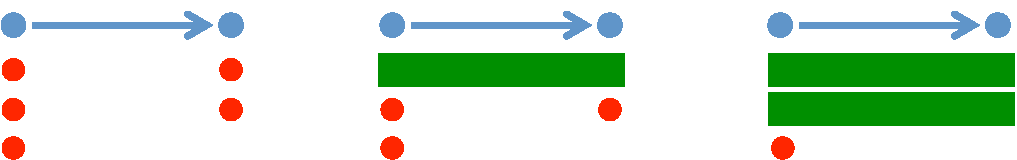
\includegraphics[width=.8\textwidth]{rank_bcs.pdf}
    \caption{Barcodes associated to $T:\R^3\to\R^2$ for $\rank(T)=0,1,2$}
    \label{fig:rank012bars}
\end{figure}

\begin{ex}[Barcodes for Filtrations]\index{barcode!filtration of Bott's torus}

Barcodes with longer bars appear in filtrations of topological spaces. For example, consider the standard height function on the torus $h:X\to\R$. By choosing a discrete set of points $\{t_0 < t_1,\ldots \}$ to sample the function $h$ at, we get a sequence of spaces $\{X_{\leq t_i}=h^{-1}(-\infty,t_i]\}$, which after taking homology in some degree $i\geq 0$ defines a persistence module. Such an example is depicted in Figure \ref{fig:persistence_torus}.

\[
X_{\leq t_0} \hookrightarrow X_{\leq t_1} \hookrightarrow \cdots \qquad \rightsquigarrow \qquad H_i(X_{\leq t_0};k) \to H_i(X_{\leq t_1};k) \to \cdots
\]

\end{ex}

\begin{figure}[ht]
    \centering
    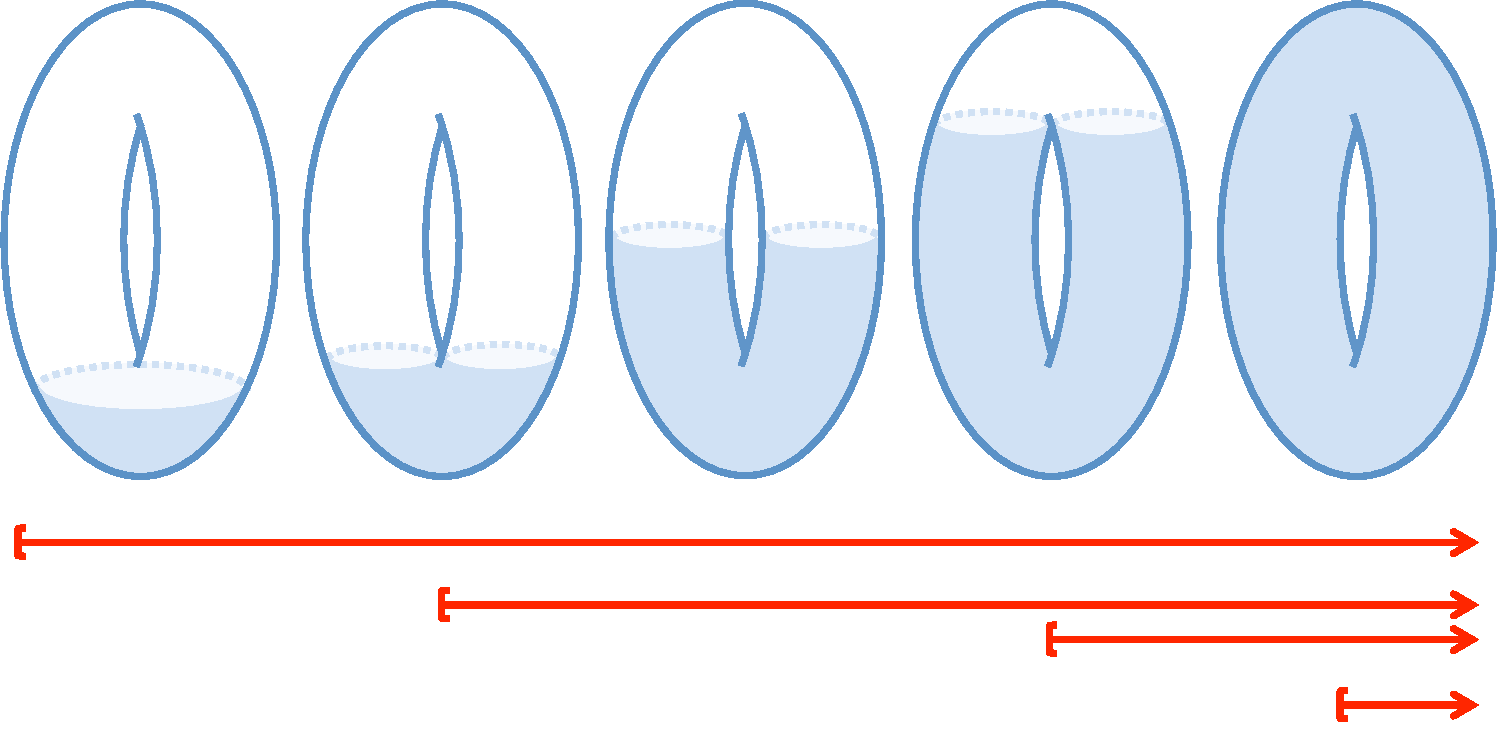
\includegraphics[width=\textwidth]{persistence_torus_ltblue.pdf}
    \caption{Barcodes for the filtration of a Torus}
    \label{fig:persistence_torus}
\end{figure}

Now we reach an example that will be useful when we undertake the derived category of chain complexes.

\begin{ex}[Barcodes for Chain Complexes]\label{ex:chaincomplex_bc}\index{barcode!associated to chain complex}
As already remarked, a chain complex of vector spaces is a special example of a persistence module and, consequently, has a barcode decomposition. With a moment's reflection one can see that any chain complex can be written as the direct sum of two types of modules: 
% \[
% V\cong \bigoplus_{i\in\ZZ} S_i^{n_i}\oplus P_i^{m_i}
% \]
the length zero interval modules
\[
S_i: \qquad \cdots \to 0 \to k \to 0 \to \cdots
\]
and the length one interval modules.
\[
P_i: \qquad \cdots \to 0 \to k \to k \to 0 \to \cdots
\]
Figure~\ref{fig:chaincomplex_bcs} gives a visual depiction of such a barcode decomposition.
\end{ex}

\begin{figure}[ht]
    \centering
    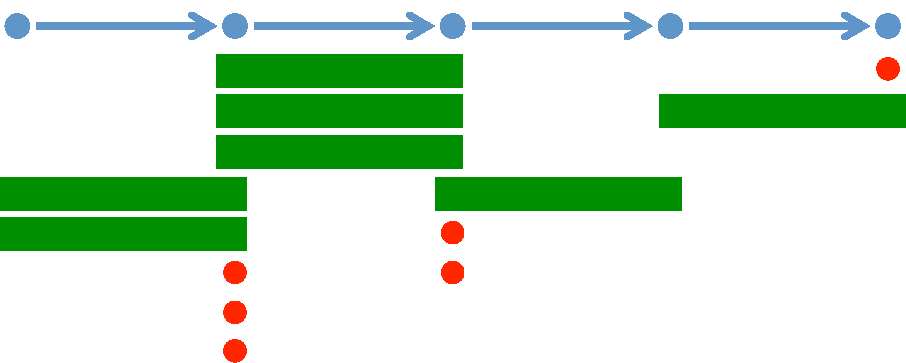
\includegraphics[width=.8\textwidth]{chaincomplex_bcs.pdf}
    \caption{Barcodes for a Chain Complex}
    \label{fig:chaincomplex_bcs}
\end{figure}


\subsection{Representation Theory of Categories and the Abelian Structure}
\label{subsubsec:rep_abs}
For the purposes of this section, there is no real difference between cellular sheaves and cosheaves --- they are both representations of the cell category $\Cell(X)$. Recall, for any category $\cat$ the \textbf{category of representations} is defined to be the category of functors to $\Vect$:\index{category!of representations}
\[
	\Rep(\cat):=\Fun(\cat,\Vect)
\]
This category has the structure of an abelian category, which we explain in this section. In effect, this means we can do everything in $\Rep(\cat)$ that we can do in $\Vect$: take kernels and cokernels of maps between representations, talk about images of maps, add maps and so on. We will introduce these properties as we need them.

\begin{clm}\index{category!exact}
	For $\cat$ a category, $\Rep(\cat)$ is an \textbf{exact category}. This means we can talk about exact sequences. Specifically:
	\begin{itemize}
		\item There is a \textbf{zero representation} given by sending all objects and morphisms to the zero object and the zero morphism.
		\item Between any two representations $F$ and $G$ there is a \textbf{zero map}, which can be factored through the zero representation.
		\item Since any morphism $\eta:F\to G$ is a natural transformation occurring inside $\Vect$, there are associated \textbf{kernel and cokernel representations} denoted $\ker(\eta)$ and $\coker(\eta)$ defined by taking kernels and cokernels object wise:
		\[
		\xymatrix{\ker(\eta(c')) \ar[r] & F(c') \ar[r]^{\eta(c')} & G(c') \ar[r] & \coker(\eta(c')) \\
		\ker(\eta(c)) \ar[r] \ar@{.>}[u] & F(c) \ar[r]^{\eta(c)} \ar[u]_{F(f)} & G(c) \ar[r] \ar[u]_{G(f)} & \coker(\eta(c)) \ar@{.>}[u] }
		\]
		\item There is an \textbf{image representation} $\im(\eta)$ defined as the object-wise image.
	\end{itemize}
\end{clm}

As usual, we say that a sequence of representations $A\to B \to C$ is \textbf{exact}\index{exact!sequence of representations} at $B$ if the kernel of the outgoing morphism is equal to the image of the incoming morphism. A longer sequence is exact if it is exact at each place with an incoming and outgoing morphism.

We are going to do a brief sketch of some representation theory for categories, using the terminology introduced.

\begin{defn}\index{representation!subrepresentation}
	A \textbf{subrepresentation} $E$ consists of a choice of subspace $E(c)\to F(c)$ for each object that is invariant under all the linear maps $F(f)$. Restriction of $F(f)|_{E(c)}=:E(f)$ makes $E$ into a representation of its own right. Said more succinctly, $E\to F$ is a natural transformation of functors that is object wise an inclusion, i.e.
	\[
		0 \to E \to F
	\] 
is an exact sequence. Dually, we can say $G$ is a quotient representation by saying $F\to G \to 0$ is an exact sequence.
\end{defn}

\begin{defn}\index{representation!direct sum}
	Suppose $F:\cat\to\Vect$ and $G:\cat\to\Vect$ are two representations of a small category $\cat$, then we can define the \textbf{direct sum} of these two representations $H=F\oplus G$ by defining on objects $H(c):=F(c)\oplus G(c)$ and on morphisms $H(f)=F(f)\oplus G(f):H(c)\to H(c')$.
\end{defn}

The above definition further clarifies the structure of $\Rep(\cat)$.

\begin{clm}\index{category!additive}\index{category!abelian}
	For $\cat$ a category, $\Rep(\cat)$ is both an exact and an \textbf{additive category}. This latter definition requires the following:
	\begin{itemize}
		\item For any two representations $F$ and $G$ the set $\Hom_{\Rep(\cat)}(F,G)$ has the structure of an abelian group (with the zero map being the additive identity) making composition bilinear.
		\item The direct sum of two representations is a representation.
	\end{itemize}
	A category that is exact and additive is defined to be \textbf{abelian}. Thus $\Rep(\cat)$ is an abelian category. 
\end{clm}

\begin{rmk}
In any additive category, it can be shown that having finite direct sums (finite coproducts) implies the existence of finite direct products (finite products) and these are isomorphic. 
\end{rmk}

\begin{defn}[Indecomposable]\index{representation!indecomposable}\index{indecomposable representation}
	A representation $F:\cat\to\Vect$ is called \textbf{indecomposable} if whenever $F$ is written as a direct sum of representations one of the representations is the zero one; i.e. every direct sum decomposition is trivial.
	
	Said using sequences, a representation $F$ is indecomposable if whenever we have a short exact sequence of representations
	\[
	0\to E \to F \to G \to 0
	\] 
	with neither $E$ nor $G$ the zero representation, then $F\ncong E\oplus G$, i.e. the sequence does not split.
\end{defn}

\begin{exr}
Verify that the interval modules in Definition \ref{defn:interval} are indecomposable representations. What is the underlying category that these modules represent?
\end{exr}

\begin{rmk}[Splitting Lemma]\index{splitting lemma}
There is a general lemma called the \textbf{splitting lemma}, which provides equivalent ways of saying that $F$ is indecomposable. It states that writing $F$ as a direct sum is equivalent to either having a map back from $F$ to $E$, which precomposed with the inclusion $E\to F$ yields the identity, or having a map back from $G$ to $F$, which post-composed with the surjection is the identity on $G$.
\end{rmk}

\begin{defn}[Remak Decomposition]\index{decomposition!Remak}
	A direct sum decomposition of an object $F\in\Rep(\cat)$
	\[
		F\cong F_1\oplus\cdots\oplus F_n
	\]
	where each $F_i$ is indecomposable and non-zero is called a \textbf{Remak decomposition}.
\end{defn}

A fact that we would very much like to know is whether every representation admits a Remak decomposition. The structure theorem \ref{thm:crawleyboevey} provides an example where this is the case. Sir Michael Atiyah considered such a question in the very general setting of abelian categories~\cite{atiyah_ks}. He developed a bi-chain condition and proved that under this condition every non-zero object admitted a Remak decomposition. We use a stronger condition of finite-dimensionality that Atiyah showed implied his bi-chain condition.

\begin{thm}[Krull-Schmidt Theorem for Representations~\cite{atiyah_ks}]\index{Krull-Schmidt Theorem}
	Suppose $\aat$ is an abelian category, further satisfying
	\begin{enumerate}
		\item For every pair of objects $\Hom_{\aat}(A,B)$ is a finite dimensional vector space, and
		\item Conjugation is linear, i.e. for every pair of morphisms $\varphi:A\to B$ and $\psi:B'\to A'$ the following map is linear
		\[
			\Hom_{\aat}(B,B')\to \Hom_{\aat}(A,A') \qquad \eta\mapsto \psi\circ\eta\circ\varphi
		\]
	\end{enumerate}
		then the Krull-Schmidt theorem holds. This says that every non-zero object $A$ has a Remak decomposition and for any two such decompositions
		\[
			A\cong A_1\oplus\cdots\oplus A_n \qquad A\cong A'_1\oplus\cdots\oplus A'_m
		\]
		$n=m$ and after re-ordering $A_i\cong A_i'$.
\end{thm}

For $\aat=\Rep(\cat)$ the second condition is certainly satisfied. The first condition imposes significantly stronger conditions. First of all, we must restrict to the full subcategory of finite dimensional representations.
\[
	\Rep_f(\cat):=\Fun(\cat,\vect) \subset \Fun(\cat,\Vect)=:\Rep(\cat)
\]
Secondly, one must observe that for any two representations $F$ and $G$ the space of natural transformations is a subspace of a potentially infinite product of finite dimensional spaces.
\[
	\Hom(F,G)\subseteq \prod_{c\in\cat}\Hom_{\vect}(F(c),G(c)) 
\]
One severe restriction one can make to insure that Atiyah's first condition holds is to assume that the category $\cat$ has finitely many objects. This is not strictly necessary, but it does provide us with the following corollary:

\begin{cor}[Sheaves and Cosheaves on Finite Posets have Remak Decompositions]\label{cor:sheaves_remak}
	Suppose $(X,\leq)$ is a finite poset, then $\Shv(X)$ and $\Coshv(X)$ satisfy the Krull-Schmidt theorem.
\end{cor}

The example that we have in mind, of course, is the poset associated to a a cell complex $X$. In this situation, one can recognize a large set of examples of indecomposable representations.

\begin{lem}[Constant (Co)Sheaves are Indecomposable]\label{lem:const_indecomp}\index{indecomposable representation!constant (co)sheaves on connected}
	Suppose $X$ is a connected cell complex, then the constant sheaf $k_X$ and the constant cosheaf $\hat{k}_X$ are indecomposable.
\end{lem}
\begin{proof}
	We'll state the proof for sheaves and leave it to the reader to dualize for cosheaves. Suppose for contradiction that $k_X\cong F\oplus G$ where neither $F$ nor $G$ is the zero sheaf. Now as a consequence of neither $F$ nor $G$ being zero, and $k_X$ being one dimensional on each cell, there must be a pair of cells $\sigma$ and $\tau$ such that one is in the support of $F$ and the other is in the support of $G$. We argue that we can choose $\sigma$ and $\tau$ such that one is the face of the other. If not, then the support of $F$ (or $G$) would be closed under the following operations
	\[
		\sigma\subset \supp(F) \quad \mathrm{and} \quad \tau\subset \bar{\sigma} \quad \mathrm{or} \quad \sigma \subset \bar{\tau} \qquad \mathrm{then} \qquad \tau\subset \supp(F)
	\]
	which by connectedness of $X$ would imply that $\supp(F)=X$; a contradiction to the supposition that neither $F$ nor $G$ was the zero sheaf. (To see why $\supp(F)=X$, one can imagine drawing the Hasse diagram of the poset $X$ and realizing that connectedness means that the diagram is connected.) Thus we have such a pair $\sigma\subset \tau$ with one in the support of $F$ and the other in the support of $G$, but this also can not occur since the identity cannot be written as a sum of zero maps.
	\[
		k\to k \neq (k\to 0)\oplus (0\to k).
	\]
\end{proof}

\subsection{Quiver Representations and Gabriel's Theorem}
\label{subsubsec:quivers}

\begin{quote}
{\em ``These graphs arise in a multitude of classification problems in mathematics, such as classification of simple Lie algebras, singularities, platonic solids, reflection groups, etc. In fact, if we needed to make contact with an alien civilization and show them how sophisticated our civilization is, perhaps showing them Dynkin diagrams would be the best choice!''}~\cite{etingof_rep}
\end{quote}

There are natural examples of representations of categories where these ideas and their consequences have been studied. One such example is the category associated to a directed graph. 

\begin{defn}\index{quiver}
A \textbf{quiver} or \textbf{directed graph} is defined by a pair of sets consisting of ``edges'' $E$ and ``vertices'' $V$ along with a pair of functions $h,t:E\to V$, which we think of as denoting the head and tail of a directed edge respectively. Alternatively, a quiver can be topologically regarded as a one-dimensional cell complex equipped with a local orientation of its edges.
\end{defn}

One should be careful to note that a directed graph is not a category in and of itself, but there is a natural category associated to a directed graph, which we now define.

\begin{defn}\index{category!path/free}
To a quiver we can associate a category called the \textbf{free category} or \textbf{path category} written $\Free(X)$ . The objects are vertices and the morphisms are directed paths between vertices. Since paths are just concatenated edges, we think of the morphisms as being freely generated by the edges. We must consider simply sitting at a vertex as the identity directed path connecting the vertex to itself. 
\end{defn}

\begin{defn}\index{quiver!representation}\index{representation!of a quiver}
A \textbf{quiver representation} is thus nothing more than a functor $F:\Free(X)\to \Vect$. Because a general path is simply a sequence of edges, such a functor is equivalent to specifying a vector space for each vertex in $V$ and a linear map for each edge in $E$ that goes from the source to the target.
\end{defn}

Every finite dimensional quiver representation can be decomposed into a direct sum of indecomposable representations. However, this list can be very unwieldy. Gabriel's theorem provides an precise description of which quivers admit a finite list of indecomposable representations.

\begin{thm}[Gabriel's Theorem~\cite{derksen}]\label{thm:gabriel}\index{Gabriel's theorem}
Let $Q$ denote a quiver. The category of representations $\Rep(Q)$ has finitely many indecomposables if and only if the underlying undirected graph of $Q$ is a union of Dynkin graphs of type $A_n$, $D_n$, $E_6$, $E_7$ or $E_8$. These are depicted in Figure \ref{fig:sldd}.
\end{thm}

\begin{figure}
    \centering
    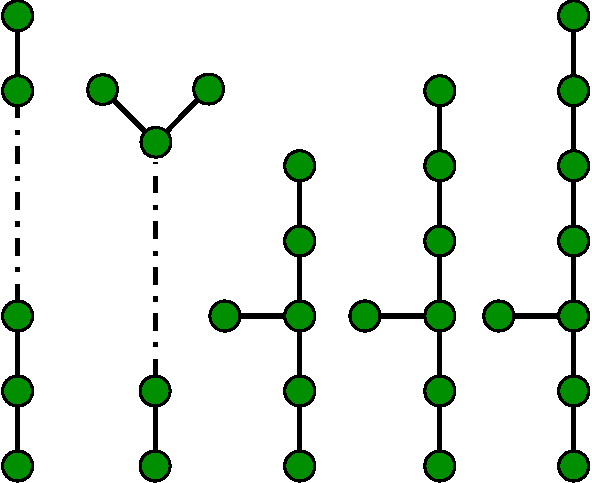
\includegraphics[width=.6\textwidth]{dynkin_diagrams.pdf}
    \caption{Simply Laced Dynkin Diagrams}
    \label{fig:sldd}
\end{figure}

\subsection{A Remark on Quivers and Perverse Sheaves}

From a quiver representation, one can always construct a cellular sheaf or cosheaf over a one-dimensional base space. This is done by turning every map
\[
	\xymatrix{F(s(e)) \ar[r]^{\rho_{t,s}} & F(t(e))}
\]
into one of the following diagrams:
\[
	\xymatrix{F(s(e)) \ar[r]^-{\rho_{t,s}} & F(t(e))=F(e) & \ar[l]_-{\id} F(t(e))} \qquad  \xymatrix{F(s(e)) & \ar[l]_-{\id} F(t(e))=F(e) \ar[r]^-{\rho_{t,s}} & F(t(e))}
\]
The former choice would make a quiver representation into a cellular sheaf, the latter into a cellular cosheaf.

There are dangers in trying to use quiver theory as a substitute for cellular sheaf or cosheaf theory. One might try to think of a poset as a certain type of quiver with vertices corresponding to elements and an edge between two elements if $s(e)\leq t(e)$. For example, consider the poset coming from the face relation of the cell complex $Y=[0,1)\times [0,1)$:
\[
	\xymatrix{ & \sigma & \\ a \ar[ur] & & b \ar[ul]\\ & x \ar[ul] \ar[uu] \ar[ur] &}
\]
A quiver representation produces a diagram of vector spaces
\[
\xymatrix{ & F(\sigma) & \\ F(a) \ar[ur] & & F(b) \ar[ul]\\ & F(x) \ar[ul] \ar[uu] \ar[ur] &}
\]
that does not commute. In contrast, if $F$ were a cellular sheaf, then the two triangles would commute. If we were to impose ``relations'' on the quiver representation by identifying different paths, then we could recover cellular sheaves. 

A relaxed version of this observation generates a combinatorial model for perverse sheaves, which was invented by Bob MacPherson~\cite{gmv} and explored by Maxim Vybornov~\cite{vybornov-mqa,vybornov-constr}.

\begin{defn}\index{perversity}
A \textbf{perversity} $p:\Z_{\geq 0} \to \Z$ is a function from the non-negative integers to the integers such that $p(0)=0$ and $p$ takes every interval $\{0,\ldots,k\}$ bijectively to an interval $\{a,\ldots,a+k\}$ where $a\in\Z_{\leq 0}$.
\end{defn}

\begin{defn}[Cellular Perverse Sheaves]\label{defn:cellular_perverse_sheaves}\index{cellular perverse sheaves}\index{sheaf!cellular perverse}
Let $X$ be a cell complex and $P_X$ its associated poset. Let $p:\Z_{\geq 0}\to\Z$ be a perversity. Define a quiver $Q_X$ whose vertices are the elements of $P_X$ and whose edges have the property that if $\tau\to\sigma$ is an edge, then $\sigma$ is incident to $\tau$ and $p(\dim\tau)=p(\dim\sigma)+1$. A \textbf{cellular perverse sheaf} assigns to each vertex of $Q_X$ a vector space $\cP(v)$ and to each edge from $\tau$ to $\sigma$ a linear map $\kappa_{\sigma,\tau}:\cP(\tau)\to\cP(\sigma)$. These maps satisfy the chain complex condition for any pair of vertices $\gamma,\tau$
\[
\sum_{\sigma} \kappa_{\gamma,\sigma}\circ \kappa_{\sigma,\tau}=0
\]
where $\sigma$ ranges over all vertices containing with an edge from $\tau$ and to $\lambda$.
\end{defn}
